\documentclass[12pt,a4paper]{article}

\usepackage[T1]{fontenc}
\usepackage{amsmath, amssymb, amsfonts}
\usepackage[magyar]{babel}
\usepackage[utf8]{inputenc}
\usepackage{graphicx}
\usepackage{graphics}
\usepackage{mathtools}
\usepackage{epsfig}
\usepackage{epstopdf}
\usepackage{cite}
\usepackage{caption}
\usepackage{hyperref}
\usepackage[bottom=4cm]{geometry}
%\geometry{a4paper, portrait, margin=1in}

\title{\huge{Alkalmazott Fizikai Módszerek Laboratórium}\\ \vspace{20pt}
\textbf{Elektronspin rezonancia}}

\author{\Large{\textsc{Csörnyei Géza}} \vspace{10pt}\\
	\textrm{Eötvös Loránd Tudományegyetem}\\
	\textrm{Fizikus MSc I}
	}
\date{}
%\lhead{}
\begin{document}
\addtolength{\voffset}{-1.0cm}
\addtolength{\textheight}{1.0cm}
\begin{titlepage}
\maketitle

\begin{figure}[!htb]
\centering

\includegraphics[scale=0.6]{eltecimer.jpg}
\end{figure}

\hfil \Large{'E' mérőcsoport}\hfil  \\
\vspace*{2pt}
\hfil \Large{\emph{Mérés dátuma:} 2019.09.27.}\hfil \\
\vspace*{2pt}
\hfil \hspace*{45pt} \Large{\emph{Mérés vezetője:} Kürti Jenő}\hfil
\thispagestyle{empty}
\end{titlepage}

\section{Bevezetés}
\hspace*{10pt} Mérésünk célja az ESR spektroszkópiai módszerrel való megismerkedés, valamint két előre elkészített mangán és króm minta ESR spektrumának felvétele volt. A felvett spektrumok segítségével kiértékelési feladatként meghatároztuk a mangán g-faktorát, a két minta hiperfinom kölcsönhatási állandóját, valamint a mintában található mangán atomok számát.

\section{Mérés elve}
\hspace*{10pt} Az elektronspin rezonancia egy olyan spektroszkópiai módszer, amellyel az elektronok energiaszintjeinek mágneses térben történő felhasadása vizsgálható. A módszer lényege, hogy sztatikus tér hatására a kialakuló Zeeman alnívók között megfelelő frekvenciájú elektromágneses hullámok segítségével átmeneteket hozunk létre. Az átmenetek létrejöttének szükséges feltétele, hogy a sztatikus feszítő tér és a gerjesztő elektromágneses tér között teljesüljön az ún. rezonancia-feltétel:
\begin{equation}
h\nu=g\mu_{B}B_0,
\end{equation}
ahol $h$ a Planck-állandó, $\nu$ a gerjesztő tér frekvenciája, $g$ a vizsgált anyag g-faktora, $\mu_{B}$ a Bohr-magneton és $B_{0}$ a sztatikus mágneses tér indukciója. A mérés során néhány tized T indukciójú mágneses térrel és (a rezonanciafeltételből következően) GHz-es nagyságrendű mikrohullámú gerjesztéssel dolgoztunk.\\
\\
\textbf{1. kérdés: Miért ilyen frekvencia- és indukciótartományban dolgoznak a tipikus ESR készülékek?}\\
\hspace*{10pt} A frekvencia- és indukciótartománynak csupán praktikai okai vannak. A létrehozott oszcilláló jelet egy hullámvezető segítségével juttatjuk a mintához, mely mérete a jel hullámhosszának nagyságrendjébe kell essen, viszont praktikai okokból nem lehet sem túl kicsi, sem túl nagy, az 1-10 cm-es mérettartomány a legpraktikusabb. Ezen felül, mivel a rezonanciafeltétel miatt rögzítve van a moduláló jel frekvenciája és a sztatikus előfeszítő tér indukciója, a mágneses tér létrehozásának nehézségeit is figyelembe kell venni. Néhány T erősségű tér létrehozható még vasmagos elektromágnesekkel, de a tér növeléséhez nagyobb elektromágnesre van szükség, efelett pedig már bonyolultabb módszerek alkalmazása szükséges. Kisebb terek esetén szintén csak praktikai okok limitálják a mérést, itt már problémás lehet a minta pontos behelyezése a mérőeszköz kisebb mérete miatt.\\
\\
\hspace*{10pt}  A hiperfinom felhasadás miatt az egyes Zeeman-szintek tovább hasadnak, emiatt az anyag magspinjétől függően több csúcsot is észlelhetünk az ESR spektrumban, ez esetben pedig a rezonancia-feltétel a következő alakot veszi fel:
\begin{equation}
h\nu=g\mu_{B}B_0+Am_{I},
\end{equation}
ahol $A$ a hiperfinom kölcsönhatási együttható, $m_{I}$ pedig a mag mágneses kvantumszáma. A fenti egyenlet értelmében tehát minden Zeeman-nívó annyi vonalra hasad, ahányféleképpen beállhat a magspin a külső sztaikus tér irányához képest.\\
\hspace*{10pt} A mérés során a sztatikus mágneses tér változtatása mellett mértük az abszorpciót (pontosabban annak deriváltját). Mivel a jel rendkívül kicsi a zaj erősségéhez képest, ezért szükséges volt egy zajszűrő technika, az ún. \emph{lock-in} módszer használata. A módszer lényege, hogy egy periodikus jelet viszünk be a mérési folyamatba, majd a kimeneti jelből kiszűrjük a pontosan ugyanígy változó komponenst, így olyan jelet kapunk, mely arányos a vizsgált és a referencia jel szorzatának bizonyos időállandóval kiátlagolt értékével. Ennek segítségével nagyon kis jelek is láthatóvá tehetők a mérés során. A méréshez 99 kHz-es lock-in jelet használtunk.\\
\\
\textbf{2. kérdés: Miért pont 99 kHz-es jelet használtunk?}\\
A jóval kisebb frekvenciájú modulálás esetében nehezebb kiszűrni a valódi jelet a zajból, emiatt nagyobb frekvenciákat választanak. A jelen értéknél jóval nagyobb frekvenciák esetében nehezebb meghatározni a jel amplitúdóját (valamint több \emph{lock-in} erősítő esetében az elérhető maximális frekvencia is ~100 kHz-es nagyságrendű). Felső határként meg van szabva az is, hogy a moduláló frekvenciának jóval kisebbnek kell lennie, mint a frekvenciaegységekben kifejezett vonalszélesség (1).

\section{Mérési elrendezés}
\hspace*{10pt} A mérés elrendezése a \ref{im-1}. ábrán látható. Az egyes eszközök rövid leírása megtalálható (2)-ben.\\
\begin{figure}[!h]
\centering
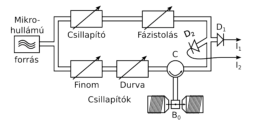
\includegraphics[scale=3]{elrend}
\caption{A mérés elrendezése}
\label{im-1}
\end{figure}
\newline
A mérést számítógépről végeztük. A mérőeszközön állítani lehetett a diódaáramot, a csillapítást, valamint a fázist, előbbi kettő beállított értéke a mangán és a króm minta esetében is 112 illetve 210 volt, míg a fázis a mangán esetén a 387, míg a króm minta esetén a 326 értékre lett beállítva.\\
\\
\textbf{3. kérdés: Miért (nem) ugyanolyan távolságra vannak a hiperfinom felhasadást szenvedett csúcsok?}\\
A (2)-ben található levezetés és a végső képlet alapján látszik, hogy a  vonalak egyenlő távolságra kell elhelyezkedjenek, hiszen a szomszédos vonalak között csak $\Delta m_I=\pm 1$ lehet a különbség. Azonban, ahogy az (2)-ben is ki lett emelve, csak a egyik komponenst vettük figyelembe az energiaszintek számításához, az erre merőleges komponenseket elhanyagoltuk. Amennyiben perturbációszámítással figyelembe vennénk azokat is, az esetben látszana, hogy eltérést okoznak, emiatt lesznek eltérések a mért vonalhelyzetek és a számolt energiaértékek között.\\
\\
\textbf{4. kérdés: Miért (nem) ugyanakkora a hiperfinom felhasadást szenvedett vonalak amplitúdói?}\\
I=1/2 magspinű atomok esetében mint például a $^1$H, a $^{19}$F vagy a $^{31}$P, ha a felhasadást ekvivalens protonok okozzák, akkor az egyes vonalak intenzitása a Pascal-háromszögnek megfelelően fog alakulni. Amennyiben nem ekvivalensek a protonok, az esetben az egyes vonalak intenzitása azonos lesz.\\
\\
\textbf{5. kérdés: H atom ESR spektruma}\\
A hidrogénatom ESR spektruma a \ref{im-h}. ábrán látható.\\
\begin{figure}[!h]
\centering
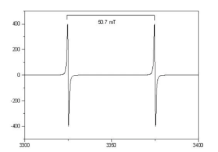
\includegraphics[scale=3]{h_spec}
\caption{A hidrogénatom ESR spektruma.}
\label{im-h}
\end{figure}
\newline
Ahogy a fenti ábrán is látszik, a hiperfinom felhasadás által két vonal jelenik meg a hidrogén ESR spektrumában, ebből következően a hidrogénatom magspinje $m_I$=1/2. A két ugyanolyan intenzitással rendelkező vonal egymástól 506.8 G-ra helyezkedik el (3).

\section{Kiértékelés}
\subsection{Mérés menete}
\hspace*{10pt} Méréseinket a mangán minta ESR spektrumának felvételével kezdtük. A mérés célja a magnézium g-faktorának és a hiperfinom kölcsönhatási együtthatójának meghatározása volt. A mérés során a mérőprogram beállításai az alábbiak voltak:
\begin{itemize}
\item{Erősítés:  0 dB}
\item{Érzékenység : 1 mV}
\item{Időállandó : 500 ms}
\item{Meredekség : 24 dB/D}
\item{Moduláló frekvencia : 99000 Hz}
\item{Moduláció amplitudója : 0.198 Gauss}
\end{itemize} Az egyes spektrumokon a mért diódaáram látható különböző sztatikus mágneses tér indukcióértékek esetére. A mangán minta esetében először olyan indukciótartományban vettük fel a spektrumot, hogy az összes hiperfinom felhasadt csúcs is biztosan látszódjon spektrumon (\ref{fig:mn_teljes}. ábra), majd nagyobb felbontással felvettük a csúcsok spektrumait is. Elegendő idő hiányában azonban csak az egyik csúcs részletes spektrumát tudtuk felvenni, ezen spektrum látható a \ref{fig:mn_csucs}. ábrán.\\
\begin{figure}[!h]
\centering
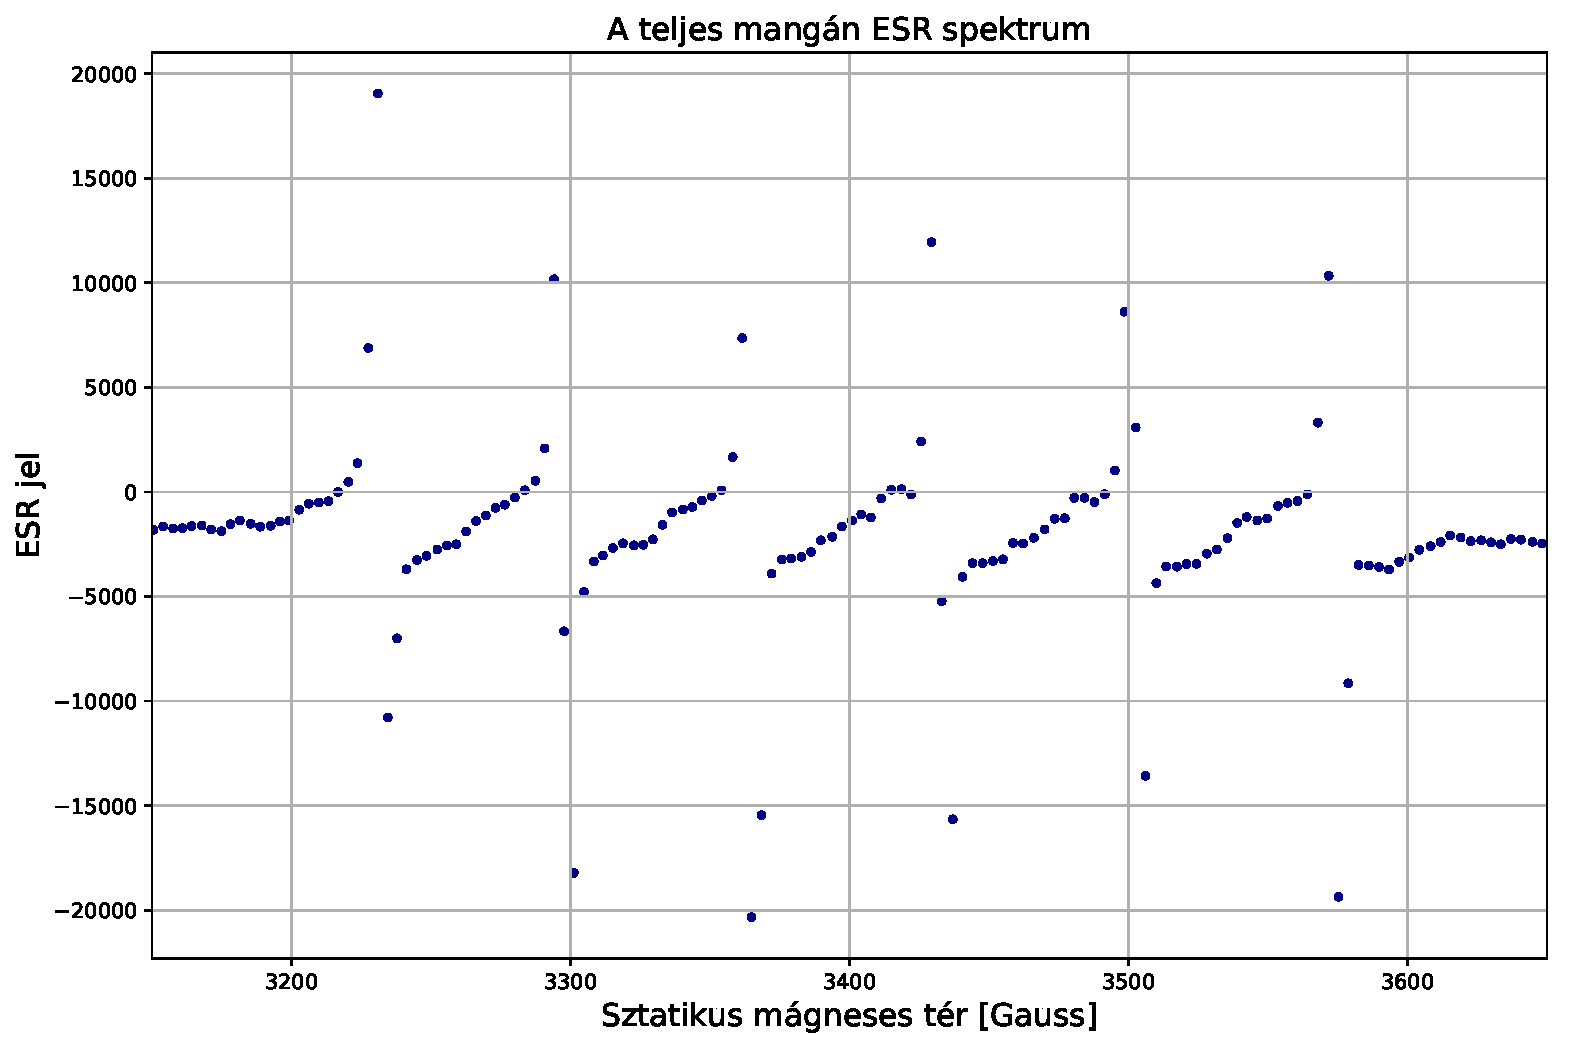
\includegraphics[scale=0.5]{mang_teljes}
\caption{A mangán minta ESR spektrumában látható csúcsok. Hat különböző csúcs látható ebben a spektrumban, ebből következően a mangán magspinje 5/2.}
\label{fig:mn_teljes}
\end{figure}
\newline
A felvett csúcsra Lorentz-görbe deriváltalakot illesztettem, melynek képlete:
\begin{equation}
f'(x)=\frac{2a(x-x_{0})}{(b^2+(x-x_{0})^2)^2},
\end{equation}
mivel a Lorentz-görbe ennek megfelelő paraméterezésű alakja:
\begin{equation}
f(x)=- \frac{a}{b^2+(x-x_{0})^2},
\end{equation}
 tehát a derivált illesztésének paramétereiből következtetni tudunk a neki megfelelő Lorentz-görbére is.\\
\begin{figure}[!h]
\centering
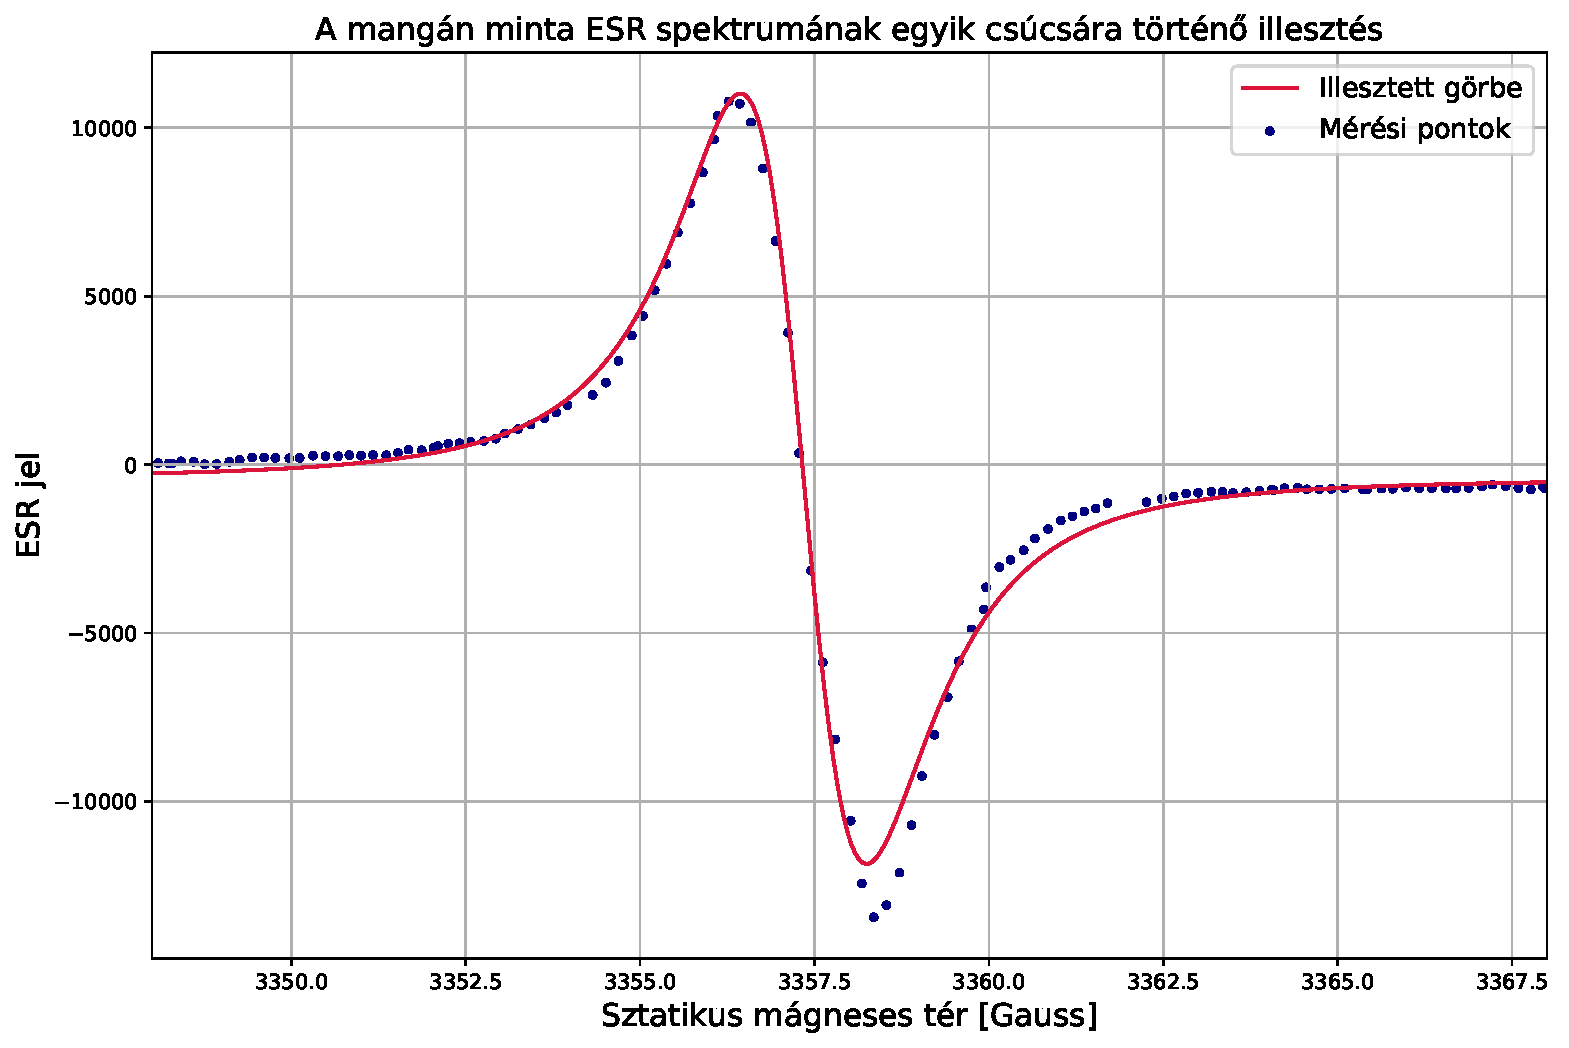
\includegraphics[scale=0.5]{mang_reszl}
\caption{A mangán minta ESR spektrumában látható egyik csúcs illesztése. A méréshez a mérőprogramon belül az érzékenységet 5 mV-ra állítottuk, a többi beállítás megfelelt a korábbinak.}
\label{fig:mn_csucs}
\end{figure}
\newline
Az illesztési paraméterek a fenti jelöléseknek megfelelően:
\begin{itemize}
\item{$a=-6.7495 \cdot 10^{4} \pm 2.179 \cdot 10^{3}$ 1/G$^2$}
\item{$b=1.565 \pm 0.019$ G}
\item{$x_0=3357.44 \pm 9.463 \cdot 10^{-3}$ G}
\end{itemize}
\newpage
A mangán g-faktorának és hiperfinom felhasadási együtthatójának kiszámításához szükségünk van a gerjesztő mágneses tér frekvenciájára is. Azonban nem csak a mangán mintán végeztünk mérést, hanem egy króm mintán is, amelyet a kalibrációra használhatunk, mivel ismert volt a benne levő krómatomok száma, valamint a króm g-faktora is. A króm minta valójában egy összetétel volt: bár első ránézésre csak egyetlen csúcs látszott a spektrumban, azonban a króm minta két különböző magspinű összetevőből állt; az egyik izotóp magspinje 3/2 volt, így négy csúcsként jelent meg a spektrumban, míg a másiknak 0 volt, ettől származott a \ref{fig:cr}. ábrán látható erős csúcs.\\
\begin{figure}[!h]
\centering
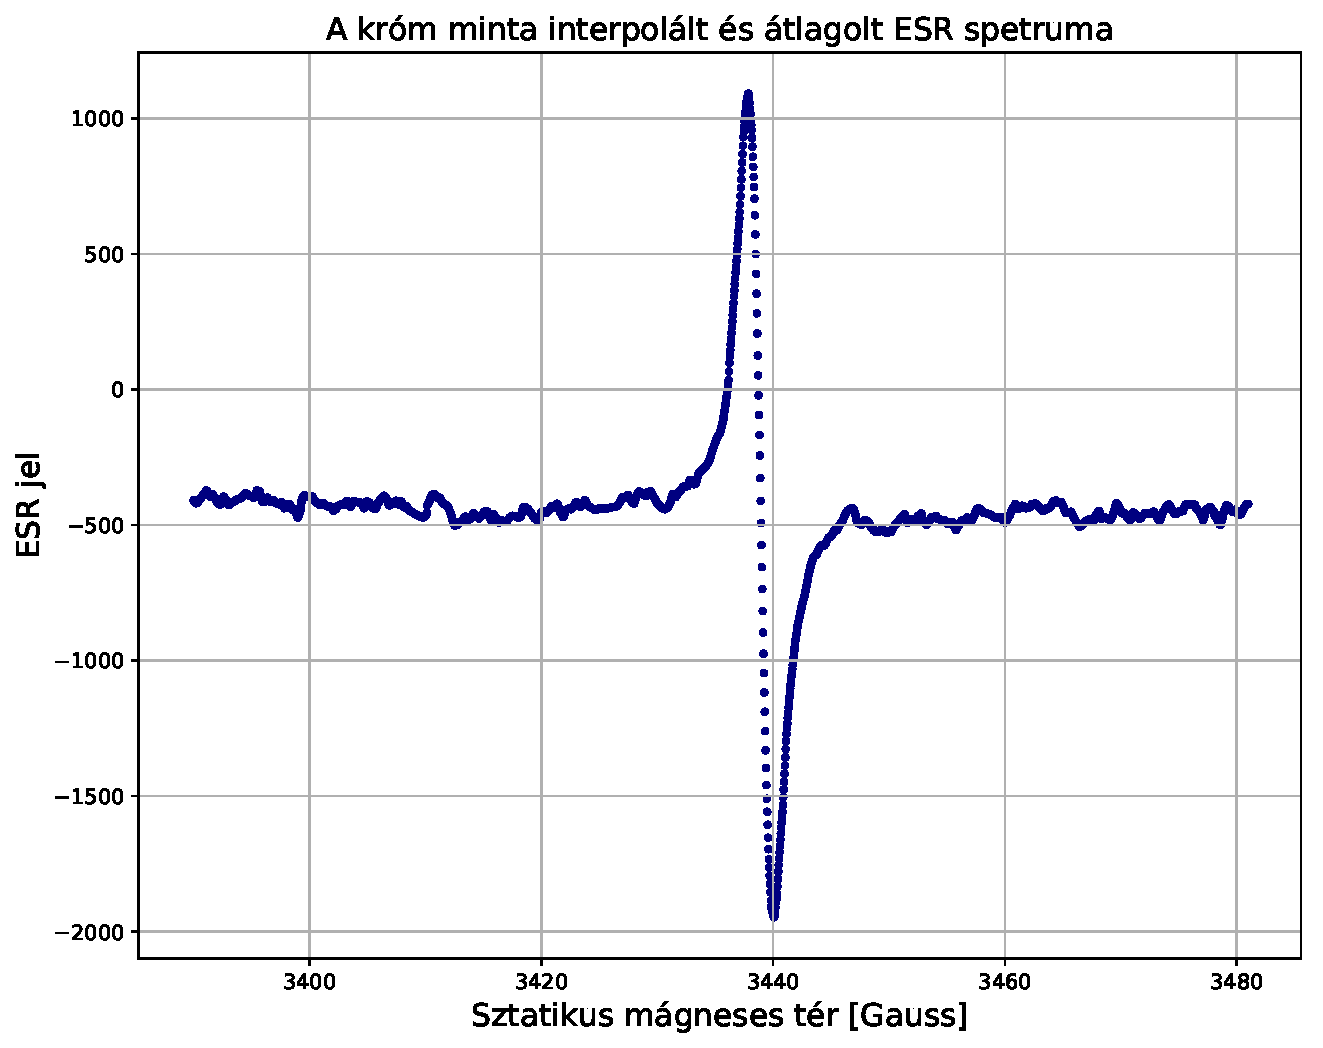
\includegraphics[scale=0.6]{crom_avg_spec}
\caption{A króm minta ESR spektruma}
\label{fig:cr}
\end{figure}
\newline
A hiperfinom felhasadást szenvedett króm izotóp hiperfinom kölcsönhatási együtthatójának meghatározásához mindenképp látnunk kellene a felhasadt csúcsokat a spektrumban. Ennek érdekében a csúcs körül három különböző mérést végeztünk, hogy ezen méréseket összeátlagolhassuk. Mivel a méréseket különböző felbontással végeztük (valamint mivel nem azonos pontokban voltak mintavételezve a spektrumok), szükséges volt az egyes spektrumok újramintavételezése, melyet lineáris interpolációval végeztem. Az egyes spektrumok 500$\mu$V-os méréshatár mellett lettek felvéve. Az interpolált spektrumokat ezek után összeátlagoltam, így kapva a fentebb látható ábrát.\\
\newpage
\hspace*{10pt} A kapott átlagspektrumra a már fentebb is látott módon Lorentz-görbe deriváltat illesztettem, hogy a görbe helyét meghatározzam. Az illesztés a \ref{fig:cr_ill}. ábrán látható.
\begin{figure}[!h]
\centering
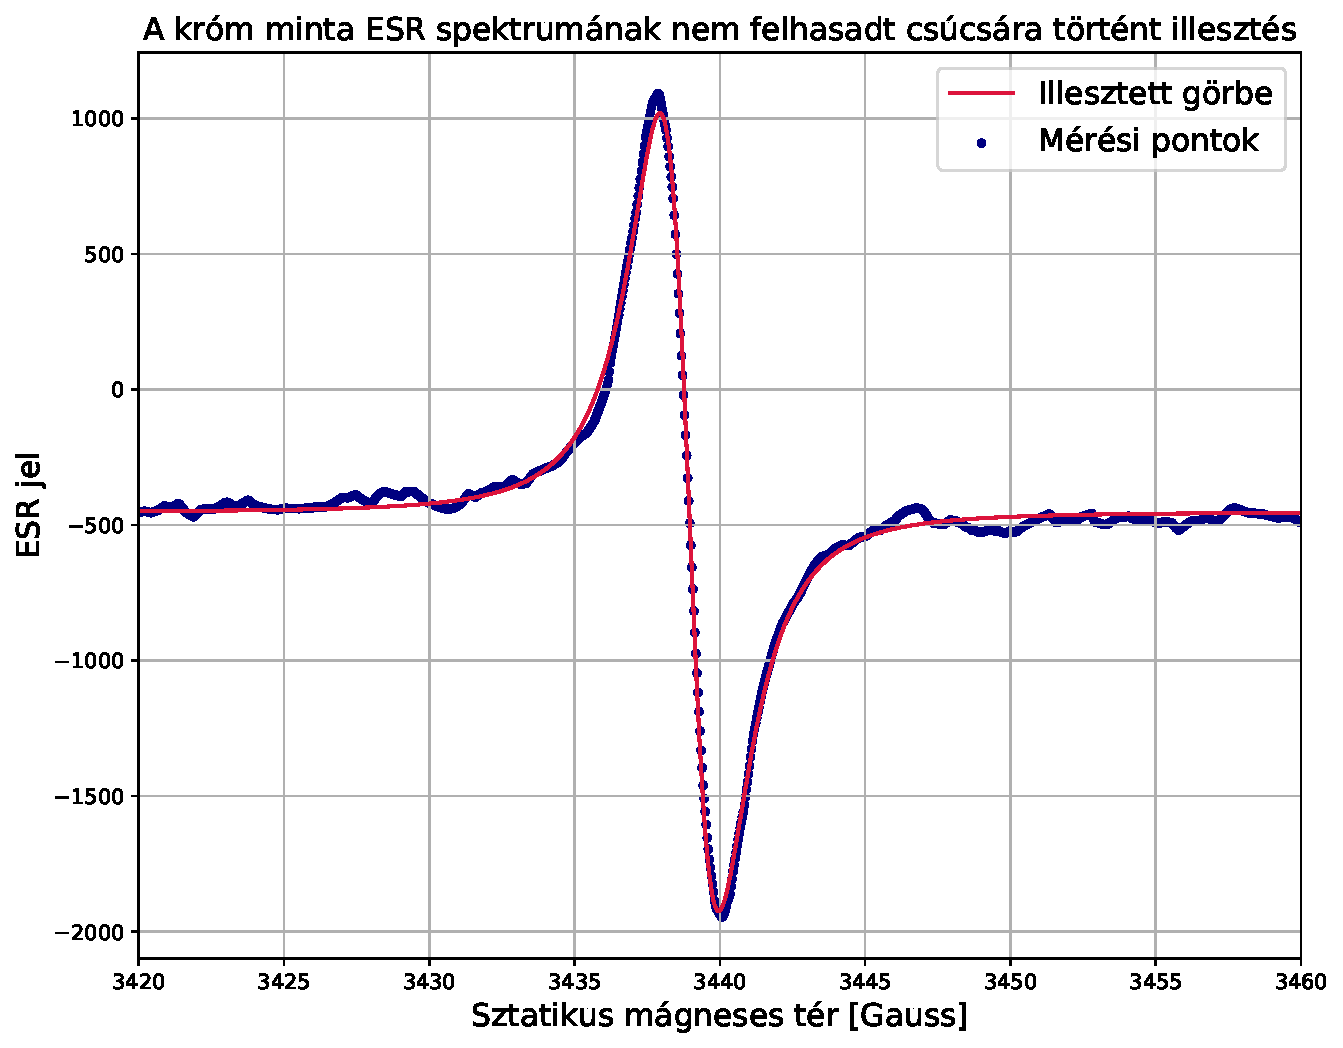
\includegraphics[scale=0.6]{cr_peak_fit}
\caption{A króm minta ESR spektrumának illesztése}
\label{fig:cr}
\end{figure}
\newline
Az illesztési paraméterek a (3) képletnek megfelelő jelöléssel:
\begin{itemize}
\item{$a=-1.213 \cdot 10^{4} \pm 8.405 \cdot 10^{1}$ 1/G$^2$}
\item{$b=1.750 \pm 4.581 \cdot 10^{-3}$ G}
\item{$x_0=3438.95 \pm 2.291 \cdot 10^{-3}$ G}
\end{itemize}
Mivel a króm g-faktorát ismertnek tekinthettük (g$_{\textrm{Cr}}$=1.98$\pm$0.0001), így használhattuk a rezonanciafeltételt a gerjesztő tér frekvenciájának meghatározásához:
\begin{equation}
\nu = \frac{g\mu_B B_0}{h}
\end{equation}
A fenti képlettel kapott frekvenciaérték $\nu=95.389 \pm 0.005$ GHz volt, ami várakozásunknak megfelelően a mikrohullámú tartományba esett. Az érték hibáját az illesztési hiba és a g-faktor relatív hibájának terjedésével számoltam. \\
\newpage
\subsection{$^{55}$Mn g-faktora és hiperfinom kölcsönhatási állandója}
A mangán g-faktorának és a hiperfinom kölcsönhatási állandójának meghatározásához szükségünk lenne hasonló illesztésekre a mangán spektrum többi csúcs esetére is, azonban idő hiányában azokról nem tudtunk spektrumot felvenni. A probléma azonban kiküszöbölhető, amennyiben azon feltevéssel élünk, hogy az egyes csúcsok formája egyforma: ekkor elegendő a fenti illesztésből kapott paraméterekkel leírt görbét elcsúsztatni más $x_0$ értékekre. Ezt úgy valósítottam meg, hogy a tejes tartomány adatsorát felosztottam a csúcsokra, majd a fenti görbét illesztettem mindegyikre úgy, hogy csak a görbe helyét hagytam meg illesztési paraméternek. Az így kapott illesztések a \ref{fig:mn_ossz}. ábrán, míg az illesztésből kapott értékek a  \ref{tab:ossz}. táblázatban láthatók.\\

\begin{figure}[!h]
\centering
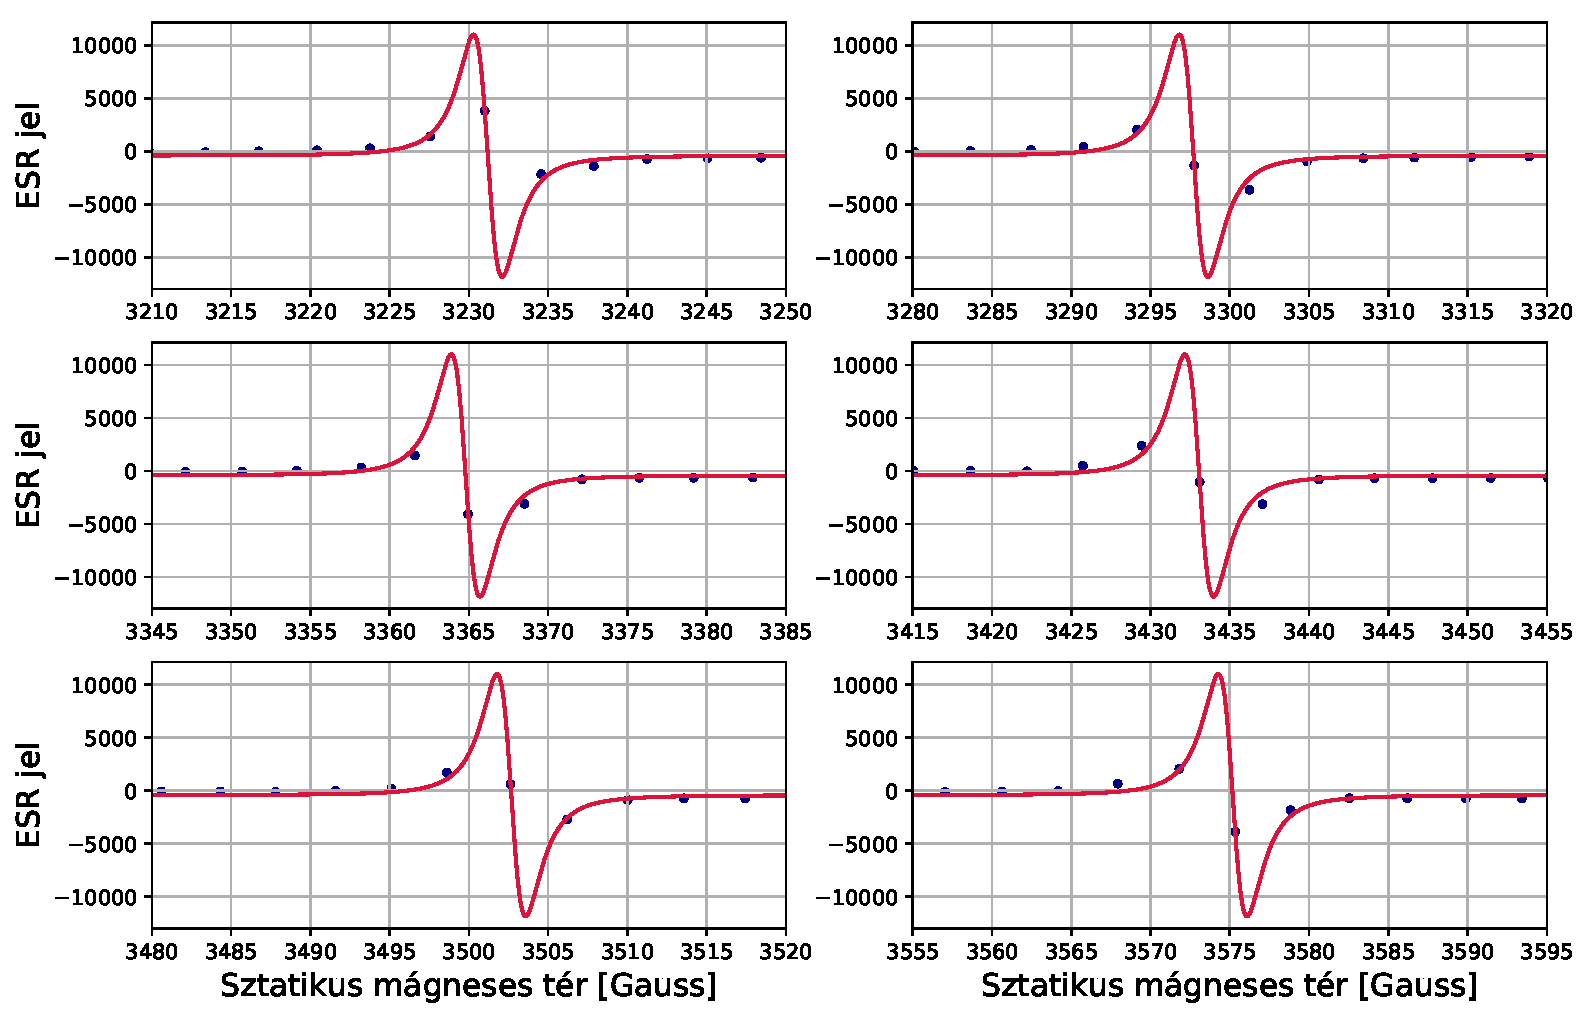
\includegraphics[scale=0.55]{mang_teljes_fits}
\caption{A mangán spektrumában látható összes csúcs illesztése}
\label{fig:mn_ossz}
\end{figure}


\begin{table}[!h]
\begin{center}
\begin{tabular}{|c|c|c|}
\hline
$m_I$ & $x_0$ [G] & $x_{0,\textrm{err}}$ [G] \\
\hline
-5/2 & 3575.181 & 0.0184 \\
\hline
-3/2 & 3502.675 & 0.0192\\
\hline
-1/2 & 3433.072 & 0.0196\\
\hline
1/2 & 3364.789 & 0.0234\\
\hline
3/2 & 3297.711 & 0.0144\\
\hline
5/2 & 3231.191 & 0.0173\\
\hline
\end{tabular}
\caption{Az illesztésből kapott sztatikus mágneses indukció értékek és azok hibái. Az egyes magspin-vetület értékeket az (2) egyenlet alapján párosítottam a mágneses indukció értékekhez (kisebb magspin értékhez nagyobb mágneses indukciót várunk a rezonanciafeltétel alapján)}
\label{tab:ossz}
\end{center}
\end{table}

\newpage
Az \ref{tab:ossz}. táblázatban található értékekre a rezonanciafeltétel alapján $B_0(m_I) = b-a\cdot m_I$ alakú egyenest illesztettem, ugyanis a rezonanciafeltétel alapján 
\begin{equation}
B_0(m_I)=\frac{1}{g\mu_B}(h\nu-Am_I).
\end{equation}
Az így végzett illesztés a \ref{fig:mn_illesztes}. ábrán látható.\\
\begin{figure}[!h]
\centering
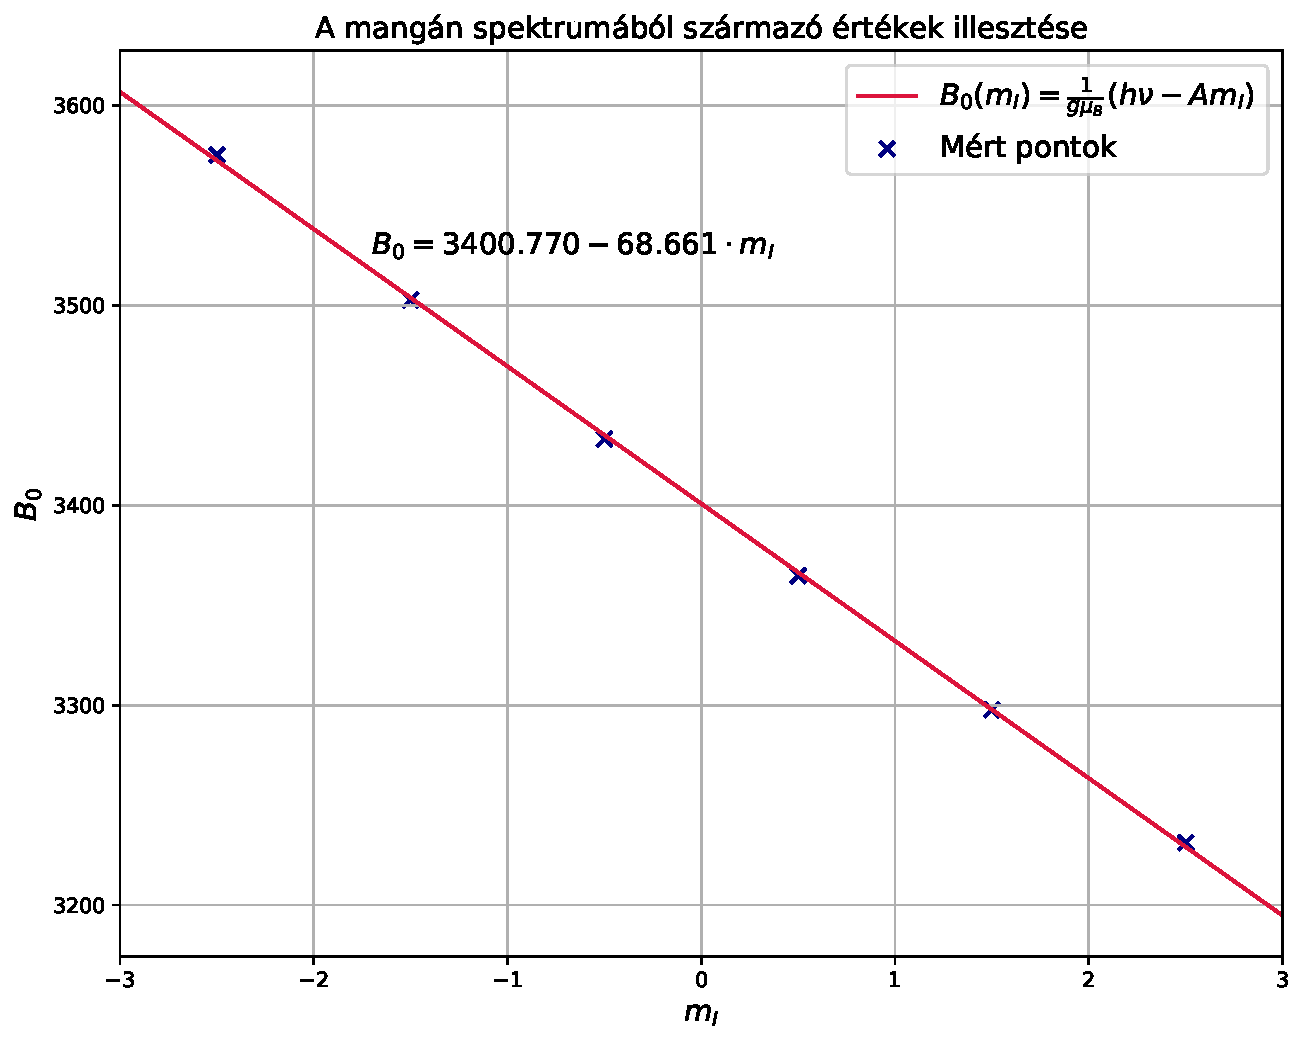
\includegraphics[scale=0.55]{mn_hf_fit}
\caption{A mangán minta adatainak illesztése a g-faktor és a hiperfinom kölcsönhatási állandó meghatározásához}
\label{fig:mn_illesztes}
\end{figure}
\newpage
Az illesztési paraméterek értékei:
\begin{itemize}
\item{$a=68.661 \pm 0.534 $ G}
\item{$b=3400.77 \pm 0.911 $ G}
\end{itemize}
Amennyiben összevetjük az elméleti és az illesztett egyenes alakját látszik, hogy $a=\frac{A}{g\mu_B}$ valamint $b=\frac{h\nu}{g\mu_B}$. Ebből következően az $^{55}$Mn g-faktora:
$$g_{\textrm{Mn}}=\frac{h\nu}{\mu_B b}=2.00267 \pm 0.00055, $$
valamint hiperfinom felhasadási együtthatója:
$$A_{\textrm{Mn}}=ag\mu_B = 1.275\cdot 10^{-25} \pm 9.918 \cdot 10^{-28} \textrm{ J}. $$

\subsection{$^{53}$Cr hiperfinom kölcsönhatási együtthatója}
\hspace*{10pt} A hiperfinom kölcsönhatási állandó számításához először detektálnunk kell a felhasadt csúcsokat. A kiátlagolt spektrumon (\ref{fig:cr}. ábra) olyan kitüremkedésket kerestem, melyek egymástól egyelő távolságra vannak. Ezen keresést kézi leolvasással végeztem, ennek megfelelően értelemszerűen nagyobb hibát kell becsülni. A leolvasott értékeket és a becsült hibát, melyben figyelembe vettem a csúcs láthatóságát, a \ref{tab:cr}. táblázat tartalmazza.\\

\begin{table}[!h]
\begin{center}
\begin{tabular}{|c|c|c|}
\hline
$m_I$ & $x_0$ [G] & $x_{0,\textrm{err}}$ [G] \\
\hline
-3/2 & 3411.89 & $\pm 0.5$ \\
\hline
-1/2 & 3430.01 & $\pm 0.7$\\
\hline
1/2 & 3447.03 & $\pm 0.7$\\
\hline
3/2 & 3465.66 & $\pm 0.5$\\
\hline
\end{tabular}
\caption{A króm minta ESR spektrumából leolvasott értékek}
\label{tab:cr}
\end{center}
\end{table}

A táblázatban a korábbihoz hasonló módon egyenest illesztettem, mely illesztés a \ref{fig:cr_ill}. ábrán látható.\\

\begin{figure}[!h]
\centering
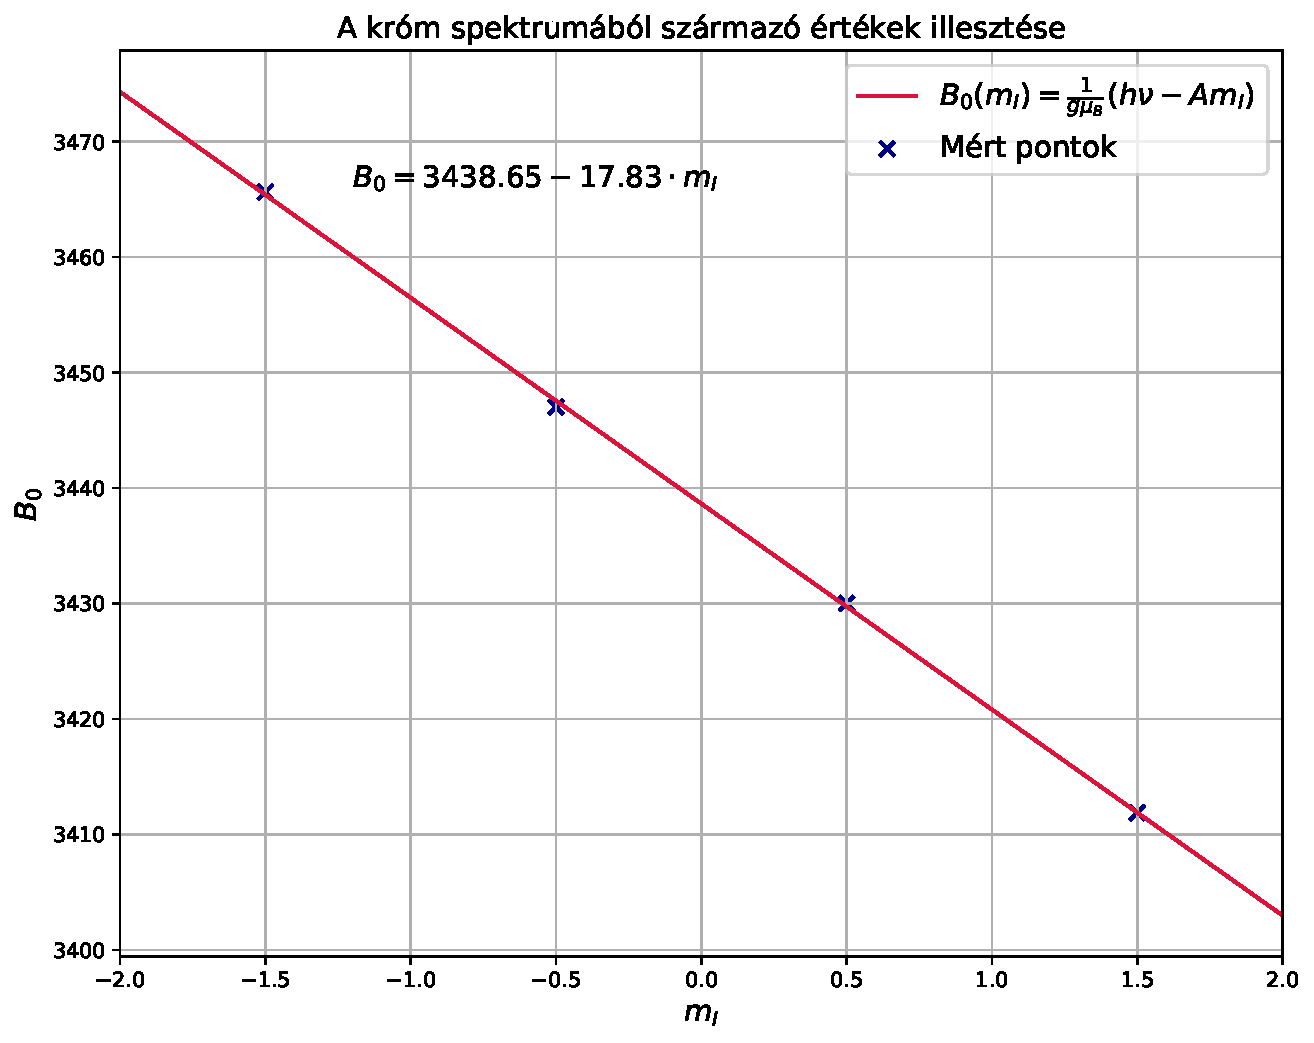
\includegraphics[scale=0.5]{cr_fl_fit}
\caption{A króm finomszerkezeti együtthatójának meghatározásához készített illesztés}
\label{fig:cr_ill}
\end{figure}
\newpage
Az illesztési paraméterek:
\begin{itemize}
\item{$a = 17.83 \pm 0.208$ G}
\item{$b = 3438.65 \pm 0.232$ G}
\end{itemize}
Ebből következően a $^{53}$Cr hiperfinom kölcsönhatási együtthatója:
$$A_{\textrm{Cr}}=ag\mu_B=3.274\cdot 10^{-26} \textrm{ J}. $$

\subsection{$^{55}$Mn atomok számának meghatározása}
\hspace*{10pt} A mérés kiértékelésének utolsó feladataként a mintában található mangán atomok számának meghatározását kaptuk. Az atomok száma egyenesen arányos az integrált ESR görbe alatti területtel, azonban a konkrét átváltási faktorokat nem ismerjük. Ennek kiküszöbölésére ismertnek tekintettük a króm mintában található atomok számát, amely $N_{\textrm{Cr}}= 8.3 \cdot 10^{13} $ volt. Amennyiben kiintegráljuk a mangán spektrumban látható csúcsok alatti területtel és ezt összevetjük a króm minta spektrumában látott csúcs alatti területtel (itt csak a nem felhasadt csúcs alatti területet veszem, a kisebbek ehhez képest elhanyagolható járulékot adnának és bizonytalan lenne az illesztésük), akkor megkapjuk a keresett atomszámot. A görbék alatti területek összevetése látható a \ref{fig:terület}. ábrán. Fontos, hogy az egyes csúcsokat azonos skálára kell állítani, mivel eltérő érzékenység mellett lettek felvéve a hozzájuk tartozó spektrumok, ennek elmulasztása torzíthatja az eredményeket.\\
\begin{figure}[!h]
\centering
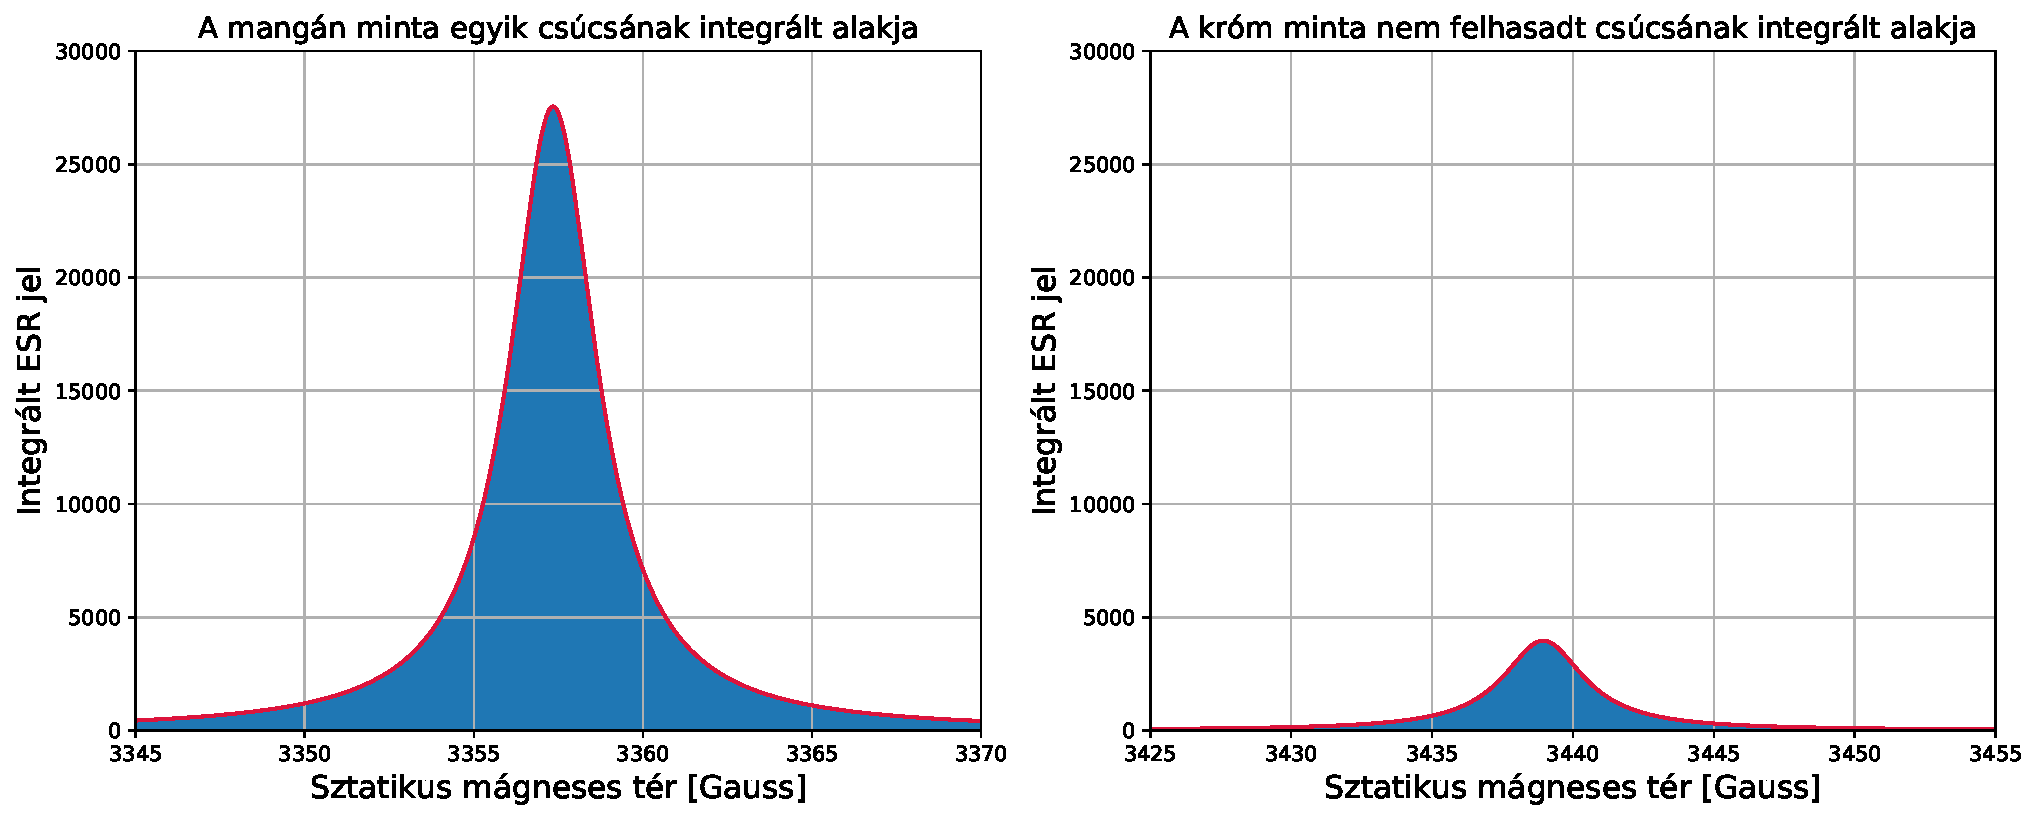
\includegraphics[scale=0.4]{int_alakok}
\caption{A csúcsok alatt területek összevetése}
\label{fig:terület}
\end{figure}
\newline
Mivel a mangán minta spektrumában hat csúcs volt, melyeket ugyanazon csúcsalakkal illesztettem meg, ezért a mangán esetében a számolt terület hatszorosát kell venni, hogy a felhasadt csúcsokat teljes egészében figyelembe vehessem. A két csúcs területének aránya (melyeket a python programcsomag numerikus integráljával számoltam) $\frac{T_{\textrm{Mn}}}{T_{\textrm{Cr}}}\approx 6.184\pm 0.142$ volt, ezáltal a mintában található mangán atomok száma:
$$N_{\textrm{Mn}}=6\cdot 6.184 \cdot N_{\textrm{Cr}} = 3.080 \cdot 10^{15} \pm 7.083 \cdot 10^{13}.$$

\section{Diszkusszió}
\hspace*{10pt} Mérésünk során sikeresen meghatároztuk a $^{55}$Mn g-faktorát, mely jó egyezést mutatott az irodalmi értékekkel, valamint meghatároztuk a kapott minták hiperfinom kölcsönhatási állandóját is. Ezen felül a mért spektrumokkal becslést is tudtunk adni a mintában található mangán atomok számára is.

\section*{Hivatkozások}
\begin{itemize}
\item[(1).:] {https://www.ph.tum.de/academics/org/labs/fopra/docs/userguide-06.en.pdf}
\item[(2).:] {http://metal.elte.hu/oktatas/alkfizlab/meresleirasok/ESRmeres.pdf}
\item[(3).:] {http://www.egyankosh.ac.in/bitstream/123456789/15798/1/Unit-11.pdf}
\end{itemize}
\end{document}
